\chapter{Matrizes e Sistemas}

Nesta unidade, discutiremos tipos especiais de matrizes, operações com matrizes e o escalonamento, também conhecido como eliminação Gaussiana. Discutiremos a fatoração $PA=LU$ e sua implementação, através de uma introdução à linguagem Python.

\section{Introdução}

A álgebra linear se preocupa principalmente com a solução de sistemas lineares. Vamos considerar primeiro o caso mais simples, em que o número de equações é igual ao número de variáveis. Considere o exemplo abaixo:
\begin{equation}
  \label{eq:sistema}
  \begin{cases}
    2x-y = 1\\
    x+y = 5.
  \end{cases}
\end{equation}
\begin{figure}[h!]
  \begin{center}
    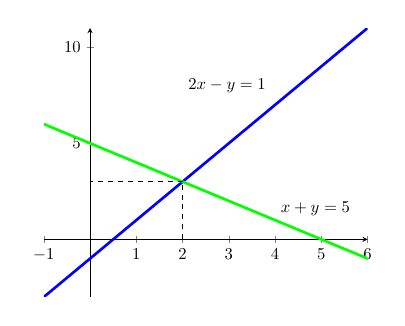
\begin{tikzpicture}[scale=0.6]
      \begin{axis}
        [
        tick scale binop=\times,
        axis x line=center, 
        axis y line=center, 
        ]
        \addplot[domain=-1:6, blue, ultra thick,samples=20] {2*x-1};
        \addplot[domain=-1:6, green, ultra thick,samples=20] {5-x};
        \addplot[black, thick, dashed] coordinates {(2,0) (2,3)};
        \addplot[black, thick, dashed] coordinates {(2,3) (0,3)};
        \draw[anchor=west] (axis cs:{2,8}) node {$2x-y=1$};
        \draw[anchor=west] (axis cs:{4,1.6}) node {$x+y=5$};
      \end{axis}
    \end{tikzpicture}
    \caption{\label{fig:sistemalinear} Resolução gráfica do sistema linear \eqref{eq:sistema}. A solução é $(x,y) = (2,3)$.}
  \end{center}
\end{figure}
É comum aprendermos duas maneiras de resolver esse tipo de problemas. A primeira é a ideia de eliminar variáveis de uma equação para resolver a outra. No exemplo, poderíamos fazer
\begin{equation*}
    \begin{cases}
        2x-y = 1\\
        x+y = 5
    \end{cases}
    \Rightarrow
    \begin{cases}
        2x-y = 1\\
        x=5-y
    \end{cases}
\end{equation*}
Substituindo o valor de $x$ na primeira equação, teremos que
\begin{equation*}
    \Rightarrow 2(5-y)-y = 1 \Rightarrow 10 - 3y = 1 \Rightarrow y = 3.
\end{equation*}
Agora, substituindo este valor de $y$ na primeira equação, deduzimos que
\begin{equation*}
    x = 5-y = 5-3 = 2.
\end{equation*}
Este método é bastante simples em um problema com poucas equações e poucas variáveis, mas não é fácil imaginar a resolução de um problema de grande porte desta forma. Da mesma forma, o segundo método, que envolve determinantes e é normalmente conhecido como \emph{regra de Cramer}, é bastante complicado e, na prática, pouco eficiente. 

Felizmente, existe uma maneira inteligente de se aplicar o primeiro método a um sistema de grande porte. O \todo{O que é um algoritmo?} algoritmo que permite a resolução de problemas desta forma e que vamos estudar é conhecido como \emph{eliminação Gaussiana.}

Já sabemos (da Geometria Analítica) que um sistema de equações do tipo
\begin{equation*}
  \begin{cases}
    a_{11}x_1+a_{12}x_2+\ldots +a_{1n}x_n=b_1\\
    a_{21}x_1+a_{22}x_2+\ldots +a_{2n}x_n=b_2\\
    \vdots\\
    a_{m1}x_1+a_{m2}x_2+\ldots +a_{mn}x_n=b_m\\
  \end{cases}
\end{equation*}
pode ser reescrito em uma forma matricial, como sendo
\begin{equation}
  \label{eq:matricial}
  Ax=b
\end{equation}
e que temos algumas possibilidades para a solução deste sistema:
\begin{itemize}
  \item Se a matriz $A$ for quadrada e inversível, então $x=A^{-1}b$, ou seja, é possível encontrarmos solução única do sistema para qualquer lado direito $b$. Em outras palavras, o sistema é possível e determinado.
  \item Se a matriz $A$ não é inversível (se não for quadrada, ou se for quadrada mas não tiver inversa), então a existência e unicidade de soluções dependem do lado direito $b$ do sistema. Para algumas escolhas de $b$ o sistema terá infinitas soluções (sistema possível e indeterminado) e para outras o sistema não terá soluções (sistema impossível). 
\end{itemize}
Para identificarmos cada um destes casos, estudaremos alguns fatos sobre as matrizes.

\section{Matrizes}

\begin{defi}
    Uma matriz é uma tabela de elementos dispostos em linhas e colunas.
\end{defi}

\begin{exemplo} Alguns exemplos de matrizes de números reais:
	\begin{equation*}
    	\begin{pmatrix}
        	1 &2 &3\\
            4 &5 &6\\
            7 &8 &9
        \end{pmatrix}, 
        \begin{pmatrix}
            2 & -1\\
            2 & 3\\
            0 & 1
        \end{pmatrix}, 
        \begin{pmatrix}
            1\\
            0\\
            3
        \end{pmatrix}, 
        \begin{pmatrix}
	        0 & 1 & -3     
        \end{pmatrix}, 
		\left( \, 2 \, \right).
    \end{equation*}
\end{exemplo}

Os elementos de uma matriz podem ser números (reais ou complexos), funções, ou ainda outras matrizes. Representamos uma matriz de $m$ linhas e $n$ colunas por
\begin{equation*}
    A_{m\times n} = \begin{pmatrix}
            a_{11} & a_{12} & \cdots & a_{1n}\\
            a_{21} & a_{22} & \cdots & a_{2n}\\
            \vdots & \vdots & \ddots & \vdots\\
            a_{m1} & a_{m2} & \cdots & a_{mn}
        \end{pmatrix} = (a_{ij})_{m\times n}.
\end{equation*}

\subsection{Tipos especiais de matrizes}

Nos exemplos abaixo, as matrizes só contém números reais. No entanto, estas definições tem equivalentes para matrizes contendo outros tipos de elemento (números complexos, funções etc).

\paragraph*{Matriz Quadrada} é aquela cujo número de linhas é igual ao número de colunas. ($m=n$).
\begin{exemplo}
    \begin{equation*}
        \left( \, 2 \, \right).
    \end{equation*}
\end{exemplo}
Neste caso, dizemos que $A$ é uma matriz de ordem $m$ (ou $n$).

\paragraph*{Matriz Nula} é aquela em que $a_{ij} = 0$ para todo $i$ e $j$.\footnote{Aqui, o correto seria dizer que $a_{ij}$ é igual ao elemento neutro da soma do conjunto onde vivem os elementos da matriz.}
\begin{exemplo}
    \begin{equation*}
        A_{2\times 2} = 
            \begin{pmatrix}
                0 & 0\\
                0 & 0
            \end{pmatrix}
			, B_{3 \times 5} =
            \begin{pmatrix}
                0 & 0 & 0 & 0 & 0\\
                0 & 0 & 0 & 0 & 0\\
                0 & 0 & 0 & 0 & 0
            \end{pmatrix}
    \end{equation*}
\end{exemplo}

\paragraph*{Matriz Coluna} é aquela que possui uma única coluna ($n=1$).

\paragraph*{Matriz Linha} é aquela que possui uma única linha ($m=1$).

\paragraph*{Matriz Simétrica} é uma matriz quadrada $A$ em que $a_{ij}=a_{ji}$, para $i=1,\ldots,m$, $j=1,\ldots,n$ ($m=n$).
\begin{exemplo}
    \begin{equation*}
        \begin{pmatrix}
           4 & 3 & -1\\
           3 & 2 & 0\\
           -1 & 0 & 5
        \end{pmatrix}
    \end{equation*}
\end{exemplo}

\paragraph*{Matriz Diagonal} é uma matriz $A$ em que os únicos elementos (possivelmente) não-nulos são os elementos $a_{ij}$ com $i=j$, $i=1,\ldots,m$, $j=1,\ldots,n$. 
\begin{exemplo}
    \begin{equation*}
        \begin{pmatrix}
        	7 & 0 & 0 & 0\\
            0 & -1 & 0 & 0\\
            0 & 0 & 2 & 0
        \end{pmatrix}
    \end{equation*}
\end{exemplo}

\paragraph*{Matriz triangular} é uma matriz quadrada em que todos os elementos abaixo (ou acima) da diagonal são nulos. 
\begin{exemplo}[Matriz Triangular Superior]
    \begin{equation*}
        \begin{pmatrix}
                2 & -1 & 0\\
                0 & -1 & 4\\
                0 & 0 & 3
        \end{pmatrix}
    \end{equation*}
    Neste caso, $a_{ij}=0$ para todo $i>j$.
\end{exemplo}

\begin{exemplo}[Matriz Triangular Inferior]
    \begin{equation*}
        \begin{pmatrix}
            2 &  0 & 0\\
           -1 & -1 & 0\\
            3 &  2 & 1
        \end{pmatrix}
    \end{equation*}
    Neste caso, $a_{ij}=0$ para todo $i<j$.
\end{exemplo}

\paragraph*{Matriz esparsa} é uma matriz que contem muitos elementos nulos. 

Não existe uma definição precisa de matriz esparsa. Quando falamos de matrizes esparsas, em geral estamos falando de matrizes que possuem menos da metade de seus elementos não-nulos, ou que possuem algum tipo de estrutura especial que concentra seus elementos não-nulos.
\begin{exemplo}
    Matrizes diagonais são esparsas.
\end{exemplo}
\begin{exemplo}
    \begin{equation*}
        \begin{pmatrix}
            1 & 0 & 0 & 2 & 0\\
            0 & 0 & 2 & 1 & 0\\
            0 & 0 & 1 & 0 & 0\\
            1 & 0 & 0 & 0 & 0\\
            0 & 1 & 0 & 0 & 1
        \end{pmatrix}
    \end{equation*}
\end{exemplo}

\paragraph*{Matriz de banda} é uma matriz esparsa cujos elementos não-nulos estão concentrados próximos à sua diagonal principal.

\begin{exemplo}
    \begin{equation*}
        \begin{pmatrix}
            2 & -1 & 0 & 0 & 0\\
            -1 & 2 & -1 & 0 & 0\\
            0 & -1 & 2 & -1 & 0\\
            0 & 0 & -1 & 2 & -1\\
            0 & 0 & 0 & -1 & 2
        \end{pmatrix}
    \end{equation*}
    A \emph{largura da banda} desta matriz é 3.
\end{exemplo}

\begin{exemplo}
    \begin{equation*}
        \begin{pmatrix}
            1 & 0 & 0 & 0 & 0\\
            1 & 1 & 0 & 0 & 0\\
            0 & 1 & 1 & 0 & 0\\
            0 & 0 & 1 & 1 & 0\\
            0 & 0 & 0 & 1 & 1
		\end{pmatrix}
    \end{equation*}
    Esta matriz é uma matriz de banda, de largura 2. Também é uma matriz triangular inferior.
\end{exemplo}

\section{Operações com matrizes}

\subsection{Adição de matrizes}

A soma de duas matrizes de mesma ordem $A_{m\times n} = (a_{ij})$ e $B_{m\times n}=(b_{ij})$ é uma matriz $m\times n$ denotada por $A+B$ cujos elementos são somas dos elementos correspondentes de $A$ e de $B$, ou seja
\begin{equation*}
    A+B = (a_{ij}+ b_{ij})_{m\times n}.
\end{equation*}

\begin{exemplo}
    \begin{equation*}
        \begin{pmatrix}
            1 & -1\\
            4 & 0 \\
            2 & 5 
        \end{pmatrix}
        +
        \begin{pmatrix}
            0 & 4\\
            -2 & 5\\
            1 & 0
        \end{pmatrix}
        =
        \begin{pmatrix}
            1 & 3\\
            2 & 5\\
            3 & 5
        \end{pmatrix}
    \end{equation*}
\end{exemplo}

\paragraph*{Propriedades} A maneira como a adição de matrizes foi definida garante que ela possuirá as mesmas propriedades da adição de números reais. Dadas as matrizes $A,B$ e $C$ de mesma ordem $m\times n$, temos:
\begin{itemize}
    \item[(i)] $A+B=B+A$ (comutatividade)
    \item[(ii)] $A+(B+C)=(A+B)+C$ (associatividade)
    \item[(iii)] $A+0 = A$, onde $0$ denota a matriz nula $m\times n$.
\end{itemize}

\subsection{Multiplicação por escalar}

Seja $A=(a_{ij})_{m\times n}$ e $k$ um escalar (número). Definimos o produto da matriz $A$ pelo escalar $k$ como uma nova matriz 
\begin{equation*}
    kA = (ka_{ij})_{m\times n}.
\end{equation*}

\begin{exemplo}
    \begin{equation*}
        -2 \begin{pmatrix}
            2 & 10\\
            1 & -3
           \end{pmatrix}
        =
           \begin{pmatrix}
            -4 & 20\\
            2 & -6
           \end{pmatrix}
    \end{equation*}
\end{exemplo}

\paragraph*{Propriedades} Dadas as matrizes $A,B$ de mesma ordem $m\times n$ e números $k,k_1,k_2$ escalares, temos:
\begin{itemize}
    \item[(i)] $k(A+B) = kA+kB$
    \item[(ii)] $(k_1+k_2)A = k_1A+k_2A$
    \item[(iii)] $0A = 0$, ou seja, se multiplicarmos o número $0$ pela matriz $A_{m\times n}$ obteremos a matriz nula $0_{m\times n}$.\footnote{Novamente, aqui poderíamos substituir o escalar (número) $0$ pelo elemento neutro do conjunto que estamos considerando.}
    \item[(iv)] $k_1(k_2A) = (k_1k_2)A$.
\end{itemize}

\subsection{Transposição}

Dada uma matriz $A = (a_{ij})_{m\times n}$, podemos obter uma outra matriz $A^T = (b_{ij})_{n\times m}$, cujas linhas são as colunas de $A$, ou seja, $b_{ij} = a_{ji}$. $A^T$ é denominada a \emph{transposta} de $A$.

\begin{exemplo}
    \begin{equation*}
        A = \begin{pmatrix}
              2 & 1\\
              0 & 3\\
              -1 & 4
            \end{pmatrix}
        _{3\times 2} \qquad A^T = 
            \begin{pmatrix}
                2 & 0 & -1\\
                1 & 3 & 4
            \end{pmatrix}
        _{2 \times 3}
    \end{equation*}
\end{exemplo}

\begin{exemplo}
    \begin{equation*}
        \begin{pmatrix}
            1\\
            2
        \end{pmatrix}
        ^T = \left( 1\, 2\right).
    \end{equation*}
\end{exemplo}

\begin{exemplo}
    \begin{equation*}
        B = \begin{pmatrix}
                1 & 3\\
                3 & 2
            \end{pmatrix}
        \qquad B^T = 
            \begin{pmatrix}
                1 & 3 \\
                3 & 2
            \end{pmatrix}
    \end{equation*}
\end{exemplo}

\paragraph*{Propriedades}
\begin{itemize}
    \item[(i)] Uma matriz é \emph{simétrica} se e somente se ela é igual à sua transposta.
    \item[(ii)] $\left(A^T\right)^T = A$.
    \item[(iii)] $(A+B)^T = A^T + B^T$.
    \item[(iv)] $(kA)^T = kA^T$, para todo escalar $k$.
\end{itemize}

\subsection{Produto de matrizes}

Vamos supor que temos dois alimentos, com certas quantidades de vitaminas A, B e C, definidas na seguinte tabela.

\begin{center}
    \begin{tabular}{l c c c}
        & A & B & C\\
        Alimento 1 & 4 & 3 & 0\\
        Alimento 2 & 5 & 0 & 1
    \end{tabular}
\end{center}

Se ingerirmos 5 unidades do Alimento 1 e 2 unidades do Alimento 2, quanto teremos consumido de cada tipo de vitamina?

Podemos representar esse problema em termos de matrizes da seguinte forma. As quantidades de vitamina de cada alimento podem ser representadas pela matriz
\begin{equation*}
    \begin{pmatrix}
        4 & 3 & 0\\
        5 & 0 & 1
    \end{pmatrix}
\end{equation*}
e as unidades do Alimento 1 e do Alimento 2 consumidas podem ser representadas pelo 
(ou matriz-linha)
\begin{equation*}
    \left( 5 \quad 2 \right).
\end{equation*}

Desta forma, a operação que nos fornecerá a quantidade total de cada vitamina ingerida é o produto definido por
\begin{align*}
    & \left( 5 \quad 2 \right)
        \begin{pmatrix}
            4 & 3 & 0\\
            5 & 0 & 1
        \end{pmatrix}\\
    &= \left( 5\cdot 4 + 2\cdot 5 \quad 5\cdot 3 + 2\cdot 0 \quad 5\cdot 0 + 2\cdot 1 \right)\\
    &= \left( 30 \quad 15 \quad 2\right)
\end{align*}

Ou seja, serão ingeridas 30 unidades de vitamina A, 15 de vitamina B e 2 de C.

Esta operação é definida como o produto de duas matrizes, e pode ser expresso formalmente da seguinte maneira: sejam $A = (a_{ij})_{m\times n}$ e $B = (b_{ij})_{n\times p}$. Definimos $AB = (c_{ij})_{m\times p}$, com
\begin{equation*}
    c_{ij} = \sum_{k = 1}^n a_{ik}b_{kj} = a_{i1}b_{1j} + \ldots + a_{in}b_{nj}.
\end{equation*}

Só podemos efetuar o produto de duas matrizes se o número de colunas da primeira for igual ao número de linhas da segunda.

\begin{exemplo}
    \begin{equation*}
        \begin{pmatrix}
            2 & 1\\
            4 & 2\\
            5 & 3
        \end{pmatrix}
    _{3\times 2} \cdot
        \begin{pmatrix}
            1 & -1\\
            0 & 4
        \end{pmatrix}
    _{2\times 2} = 
        \begin{pmatrix}
            2\cdot 1+1\cdot 0 & 2(-1)+1\cdot 4\\
            4\cdot 1+2\cdot 0 & 4(-1)+2\cdot 4\\
            5\cdot 1+3\cdot 0 & 5(-1)+3\cdot 4
        \end{pmatrix}
     =  
        \begin{pmatrix}
            2 & 2\\
            4 & 4\\
            5 & 7
        \end{pmatrix}
    \end{equation*}
\end{exemplo}

\begin{exemplo}
    \begin{equation*}
        \begin{pmatrix}
            1 & -1\\
            0 & 4
        \end{pmatrix}
        _{2\times 2} \cdot
        \begin{pmatrix}
            2 & 1\\
            4 & 2\\
            5 & 3
        \end{pmatrix}
        _{3\times 2}
    \end{equation*}
    Não é possível efetuar este produto.
\end{exemplo}

\paragraph*{Propriedades} 
\begin{itemize}
    \item[(i)] Em geral, $AB\ne BA$.
    \begin{exemplo}
        \begin{equation*}
            A = \begin{pmatrix}
                    1 & -1 & 1\\
                    -3 & 2 & -1\\
                    -2 & 1 & 0
                \end{pmatrix}
            , \, B =
                \begin{pmatrix}
                    1 & 2 & 3\\
                    2 & 4 & 6\\
                    1 & 2 & 3
                \end{pmatrix}
        \end{equation*}
        \begin{equation*}
            AB = \begin{pmatrix}
                    0 & 0 & 0\\
                    0 & 0 & 0\\
                    0 & 0 & 0
                \end{pmatrix}
            , \, \, BA = 
                \begin{pmatrix}
                    -11 & 6 & 1\\
                    -22 & 12 & -2\\
                    -11 & 6 & -1
                \end{pmatrix}
        \end{equation*}
    \end{exemplo}
    Além disso, $AB$ pode ser nula sem que $A$ ou $B$ sejam nulas.

    \item[(ii)] $AI = IA = A$
    \item[(iii)] $0A = 0$ e $A0 = 0$.
    \item[(iv)] Sejam $A_{m\times p}$, $B_{p\times n}$ e $C_{p\times n}$. Então, $A(B+C)$ é uma matriz com elementos dados por
   \begin{align*}
		(A(B+C))_{ij} &= \sum_{k=1}^p a_{ik} (b_{kj}+c_{kj}) \\
		&= \sum_{k=1}^p a_{ik}b_{kj}+a_{ik}c_{kj} \\
		&= \sum_{k=1}^p a_{ik}b_{kj}+\sum_{k=1}^p a_{ik}c_{kj} \\
		&= (AB)_{ij} + (AC)_{ij}.
   \end{align*}
	Logo, $A(B+C) = AB+AC$ (distributividade à esquerda da multiplicação)
    \item[(v)] $(A+B)C = AC+BC$ (distributividade à direita da multiplicação)
(análogo ao caso anterior)
    \item[(vi)] Sejam $A_{m\times p}$, $B_{p\times q}$, $C_{q\times n}$. Então, $(AB)C = A(BC)$ (associatividade da multiplicação).

    Precisamos mostrar que $((AB)C)_{ij} = (A(BC))_{ij}$. Mas, note que:
    \begin{align*}
       (A(BC))_{ij} &= \sum_{k=1}^p A_{ik} (BC)_{kj}\\
       &= \sum_{k=1}^p A_{ik} \sum_{\ell=1}^q B_{k\ell} C_{\ell j}\\
       &= \sum_{k=1}^p \sum_{\ell=1}^q A_{ik} B_{k\ell} C_{\ell j}\\
       &= \sum_{\ell=1}^q \sum_{k=1}^p A_{ik} B_{k\ell} C_{\ell j}\\
       &= \sum_{\ell=1}^q \sum_{k=1}^p (A_{ik} B_{k\ell}) C_{\ell j}\\
       &= \sum_{\ell=1}^q (AB)_{i\ell} C_{\ell j}\\
       &= ((AB)C)_{ij}.
    \end{align*}
    \item[(vii)] $(AB)^T = B^T A^T$ (Exercício!)
\end{itemize}

\subsection{4 diferentes formas de se fazer um produto de matrizes}

Podemos encarar o produto de duas matrizes como vimos anteriormente, de forma monolítica, mas existem três outros jeitos de interpretarmos esta operação.

\begin{itemize}
    \item[(i)] Cada entrada da matriz-produto $AB$ é o produto entre uma linha e uma coluna:
    \begin{equation*}
        (AB)_{ij} = \mbox{ linha } i \mbox{ de } A \mbox{ vezes a coluna } j \mbox{ de } B
    \end{equation*}
    \item[(ii)] Cada coluna de $AB$ é o produto entre uma matriz e uma coluna:
    \begin{equation*}
        \mbox{coluna } j \mbox{ de } AB = A \mbox{ vezes coluna } j \mbox{ de } B
    \end{equation*}
    \item[(iii)] Cada linha de $AB$ é o produto entre uma linha e uma matriz:
    \begin{equation*}
        \mbox{linha } i \mbox{ de } AB = \mbox{ linha } i \mbox{ de } A \mbox{ vezes } B.
    \end{equation*}
\end{itemize}

\begin{exemplo*}
  \begin{align*}
    \begin{bmatrix}
      1 & 0\\
      2 & 3
    \end{bmatrix}
    \begin{bmatrix}
      2 & 1\\
      3 & 4
    \end{bmatrix}
    &= 
    \begin{bmatrix}
      1\cdot 2+0\cdot 3 & 1\cdot 1+0\cdot 4\\
      2\cdot 2+3\cdot 3 & 2\cdot 1+3\cdot 4
    \end{bmatrix}
    \begin{pmatrix}
      \begin{bmatrix}
        1 & 0\\
        2 & 3
      \end{bmatrix}
      \begin{bmatrix}
        2\\3
      \end{bmatrix}
      &
      \begin{bmatrix}
        1 & 0\\
        2 & 3
      \end{bmatrix}
      \begin{bmatrix}
        1\\4
      \end{bmatrix}
    \end{pmatrix}\\
    &= 
    \begin{bmatrix}
      \begin{bmatrix}
        1 & 0
      \end{bmatrix}
      \begin{bmatrix}
        2 & 1\\
        3 & 4
      \end{bmatrix}\\
      \begin{bmatrix}
        2 & 3
      \end{bmatrix}
      \begin{bmatrix}
        2 & 1\\
        3 & 4
      \end{bmatrix}
    \end{bmatrix}
  \end{align*}
\end{exemplo*}

\subsection{Matriz Inversa}

\paragraph*{Matriz Identidade} é uma matriz $I_{n\times n}$ tal que para toda matriz $A_{n\times n}$,
\begin{equation*}
	AI=IA=A.
\end{equation*}

Dada $A_{n\times n}$, se pudermos encontrar uma outra matriz $B_{n\times n}$ tal que 
$$AB=BA=I,$$
então diremos que $A$ é inversível e que $B=A^{-1}$. Senão, diremos que $A$ é singular.

\begin{teo}
   A inversa de $A_{n\times n}$ é única.
\end{teo}
\bpr
	Suponha que existem duas inversas de $A$, $B$ e $C$. Então, 
	$$BA = I \Leftrightarrow (BA)C = IC = C.$$
	No entanto, 
    $$AC = I \Leftrightarrow B(AC) = BI = B.$$
    Logo, como $(BA)C=B(AC)$ pela propriedade associativa do produto de matrizes, temos que $B=C$.
\epr

\begin{teo}
   Se $A, B$ são matrizes $n\times n$ inversíveis, então $(AB)^{-1} =
B^{-1}A^{-1}$.
\end{teo}
\bpr
	Basta verificarmos que $(AB)B^{-1}A^{-1} = B^{-1}A^{-1} AB$, já que a inversa é única.
\epr

\begin{teo}
   Se $A$ é inversível, $A^T$ também o é, e $(A^T)^{-1} = (A^{-1})^T$.
\end{teo}
\bpr
	Basta verificarmos que $(A^T)(A^{-1})^T = (A^{-1})^TA^T = I$.
	
	Mas $A^T(A^{-1})^T = (A^{-1}A)^T = I^T = I$. Além disso, $(A^{-1})^TA^T = (AA^{-1})^T = I^T = I.$
\epr

\section{Fatoração $PA=LU$ de uma matriz $A$.}

\subsection{Sistemas Lineares}

Considere o sistema linear
\begin{align*}
    Ax=b \Leftrightarrow 
        \begin{pmatrix}
            a_{11} & a_{12} & \cdots & a_{1n}\\
            a_{21} & a_{22} & \cdots & a_{2n}\\
            \vdots & \vdots & \ddots & \vdots\\
            a_{m1} & a_{m2} & \cdots & a_{mn}
        \end{pmatrix}
        \begin{pmatrix}
            x_1\\
            x_2\\
            \vdots\\
            x_n
        \end{pmatrix}
        =
        \begin{pmatrix}
            b_1\\
            b_2\\
            \vdots\\
            b_m
        \end{pmatrix}
\end{align*}
em que $A_{m\times n}$ é uma matriz de números reais, $x$ é um vetor com $n$ componentes reais e $b$ é um vetor com $m$ componentes reais. Se $b = 0$, chamamos este sistema de \emph{homogêneo}.

Ideia: transformar a matriz (quadrada) geral em uma matriz triangular para resolver o sistema linear por substituição. Vamos considerar primeiramente sistemas quadrados.

\begin{exemplo*}
\begin{equation*}
	\begin{cases}
		x_1 + 2x_2 + x_3 = 1\\
		2x_1 + x_2 + x_3 = 1\\
		2x_1 - x_2 + x_3 = 1
    \end{cases}
\end{equation*}
\end{exemplo*}

\subsection{Forma matricial: Forma escalonada do sistema}

Poderíamos resolver um sistema $Ax=b$ encontrando a inversa de $A$, pois se $Ax=b$, então
\begin{equation*}
	x = A^{-1}b
\end{equation*}
No entanto, encontrar a inversa de uma matriz não é tarefa fácil; assim, vamos procurar resolver o sistema usando outras estratégias.
\begin{exemplo*}
	\begin{equation*}
		\begin{cases} 
        	x+y+2z = 9\\ 
            2x+4y-3z = 1\\ 
            3x+6y-5z = 0 
        \end{cases}
	\end{equation*}
	Inicialmente, vamos tentar eliminar $x$ na segunda e terceira equações:
	\begin{equation*}
    	\left\{
		\begin{array}{r r r l}
			x &+ y &+ 2z  &=  9\\ 
			  & y &- \frac{7z}{2}  &=  -\frac{17}{2}\\ 
			  &-y &+ \frac{11z}{3} &= 9 
		\end{array}
        \right.
	\end{equation*}
	Agora, vamos eliminar $y$ na terceira equação:
	\begin{equation*}
		\left\{ 
		\begin{array}{r r r l}
			x&+y &+ 2z &= 9\\ 
			 & y &-(7/2)z &= -17/2\\ 
			 &   & (1/6)z &= 1/2 
		\end{array} 
		\right.
	\end{equation*}
	Resolvendo para $z$, temos que 
	\begin{equation*}
    	z = 3
    \end{equation*}
	Além disso,
	\begin{equation*}
    	2y - 7z = -17 \Leftrightarrow 2y = -17+21 = 4 \Leftrightarrow y = 2
    \end{equation*}
	Por último,
	\begin{equation*}
    	x+y+2z = 9 \Leftrightarrow x = 9 -2(3)-2 = 9-8 = 1.
    \end{equation*}
\end{exemplo*}

\begin{exemplo*}
	Considere o seguinte exemplo: (homogêneo)
	\begin{equation*}
		\begin{cases}
			x_1 - 2x_2  + x_3 =0\\
			x_1+x_2+x_3=0\\
			x_1  +x_3 = 0
		\end{cases}
	\end{equation*}
	Podemos representar o processo, agora numa forma matricial:
	\begin{equation*}
		\begin{pmatrix}
			x_1 & -& 2x_2 & +&x_3&=&0\\
			x_1&+&x_2&+&x_3&=&0\\
			x_1& & &+&x_3 &=& 0
		\end{pmatrix} \rightarrow 
		\begin{pmatrix}
			x_1 & -& 2x_2 & +&x_3&=&0\\
			 &-&3x_2&&&=&0\\
			&-&2x_2 & & &=& 0
		\end{pmatrix}
	\end{equation*}
	Aqui, podemos ver que, pelas equações acima, $x_2 = 0$, $x_1+x_3 = 0$, ou seja $x_1$ é \emph{livre}, $x_2 = 0$ e $x_3 = -x_1$. Neste caso, o sistema tem infinitas soluções. 

	Se, por outro lado, o lado direito for diferente de nulo, teremos:
	\begin{equation*}
		\begin{pmatrix}
			x_1 & -& 2x_2 & +&x_3&=&1\\
			x_1&+&x_2&+&x_3&=&2\\
			x_1& & &+&x_3 &=& 3
		\end{pmatrix} \rightarrow 
		\begin{pmatrix}
			x_1 & -& 2x_2 & +&x_3&=&1\\
			 &-&3x_2&&&=&1\\
			&-&2x_2 & & &=& 2
		\end{pmatrix}
	\end{equation*}
	De onde vemos que o valor de $x_2$ não pode ser encontrado. Portanto, esse sistema é inconsistente.

	No entanto, se tivéssemos
	\begin{equation*}
		\begin{pmatrix}
			x_1 & -& 2x_2 & +&x_3&=&6\\
			x_1&+&x_2&+&x_3&=&-3\\
			x_1& & &+&x_3 &=& 0
		\end{pmatrix} \rightarrow 
		\begin{pmatrix}
			x_1 & -& 2x_2 & +&x_3&=&6\\
			 &-&3x_2&&&=&9\\
			&-&2x_2 & & &=& 6
		\end{pmatrix}
	\end{equation*}
	então o sistema seria consistente, mas teria infinitas soluções.
\end{exemplo*}

Qual é o problema que podemos encontrar aqui? {\bf{Pivôs nulos.}} Isso indica problemas no sistema. Assim, esse procedimento pode ser usado para identificar classes de sistemas lineares; se o procedimento puder ser realizado até o fim, sabemos que teremos uma solução definida para o sistema.

\subsection{Eliminação Gaussiana e a Forma Escalonada}

O procedimento que descrevemos acima é chamado de \emph{Eliminação Gaussiana}. O objetivo da eliminação gaussiana é obter a chamada \emph{forma escalonada da
matriz}. 

\begin{defi}
   Uma matriz $A$ está na forma escalonada quando:
   \begin{itemize}
      \item Se uma linha não for inteiramente nula, o primeiro número não-nulo da linha (indo da esquerda para a direita) é 1 (pivô);
		\item Se uma linha é nula, ela está abaixo de todas as linhas que contém elementos não-nulos;
		\item Para cada duas linhas não-nulas, o pivô da de baixo está mais à direita que o da de cima;
		\item Cada coluna que tem pivô é nula no resto. (se utilizarmos o procedimento de Gauss-Jordan até o final)
   \end{itemize}
\end{defi}

Esta definição é válida também para sistemas não quadrados, mas por enquanto vamos nos concentrar em sistemas quadrados. 

Para estes sistemas, temos algumas situações que podem ocorrer.

Para sistemas não-homogêneos:
\begin{itemize}
   \item Se pudermos realizar o escalonamento até o fim sem encontrarmos pivôs nulos, temos dois casos:
	\begin{itemize} 
		\item se o lado direito for consistente com as equações,
então temos um sistema consistente e determinado (caso quadrado)
		\item se o lado direito for inconsistente, não poderemos encontrar solução para o sistema.
	\end{itemize}
	\item Se não pudermos realizar o escalonamento até o fim, também temos duas situações:
	\begin{itemize}
		\item Se o lado direito for consistente, teremos um sistema consistente indeterminado (infinitas soluções)
		\item caso contrário, teremos um sistema inconsistente, sem soluções.
	\end{itemize}
\end{itemize}
Para o caso homogêneo,
\begin{itemize}
   \item Se pudermos realizar o escalonamento até o fim sem encontrarmos pivôs nulos, então a solução trivial é solução do sistema.
	\item Caso contrário, o sistema tem infinitas soluções (indeterminado).
\end{itemize}

\subsection{Operações elementares: Matrizes elementares} 

Nestes exemplos, resolvemos o sistema ao realizarmos as chamadas operações elementares nas linhas nestas matrizes. As operações elementares são:

\begin{itemize}
   \item Multiplicar uma linha por um escalar não-nulo;
   \item Trocar uma linha $r$ do sistema por $r+cs$, onde $c$ é um escalar e $s$ é outra linha do sistema ($r\ne s$);
   \item Trocar duas linhas de lugar.
\end{itemize}

Estas operações são importantes pois podem ser revertidas! Vamos analisar essas operações na forma matricial.

\begin{defi}
   Uma matriz $n\times n$ que pode ser obtida da matriz $I_n$ executando-se uma única operação elementar sobre linhas é uma matriz elementar.
\end{defi}

Se $E$ resulta de uma operação elementar em $I_{m\times m}$ e $A_{m\times n}$, então $EA$ realiza as mesmas operações em $A$.

\begin{exemplo*}
	\begin{equation*}
		E = \begin{pmatrix} 1&0&0\\0&1&0\\3&0&1 \end{pmatrix} = EI.
	\end{equation*}
	\begin{equation*}
	   A = \begin{pmatrix} 1&0&2&3\\ 2&-1&3&6\\1&4&4&0\end{pmatrix}; \qquad EA =
\begin{pmatrix} 1&0&2&3\\ 2&-1&3&6\\ 4&4&10&9\end{pmatrix}
	\end{equation*}
\end{exemplo*} 

\begin{teo}
   Toda $E$ elementar é inversível, e $E^{-1}$ também é elementar.
\end{teo}
\bpr
	Seja $E_0$ a matriz que resulta da aplicação da operação elementar
inversa de $E$ em $I$ (garantida pois estamos em um corpo!!). Então,
	$$E_0 E = I = EE_0$$
	$E_0$ também é elementar pois representa também uma operação elementar.
\epr

\begin{exemplo*}
	\begin{equation*}
	   \begin{pmatrix} 2&1&1\\4&-6&0\\-2&7&2 \end{pmatrix} \qquad b =
\begin{pmatrix} 5\\-2\\9 \end{pmatrix}
	\end{equation*}
	Temos então, na sequência:
	\begin{eqnarray*}
		E^{(1)}  A & = & A^{(1)}\\
		\begin{pmatrix}
			1&0&0\\-2&1&0\\0&0&1
		\end{pmatrix}
		\begin{pmatrix}
			2&1&1\\4&-6&0\\-2&7&2
		\end{pmatrix}
		&
		=
		&
		\begin{pmatrix}
			2&1&1\\0&-8&-2\\-2&7&2
		\end{pmatrix}
	\end{eqnarray*}
	Além disso, 
	\begin{eqnarray*}
	   E^{(1)} b &=& b^{(1)}\\
		\begin{pmatrix}
			1&0&0\\-2&1&0\\0&0&1
		\end{pmatrix}
		\begin{pmatrix}
			5\\-2\\9
		\end{pmatrix}
		&=&
		\begin{pmatrix}
			5\\-12\\9
		\end{pmatrix}
	\end{eqnarray*}
	Continuando o processo, 
	\begin{eqnarray*}
		E^{(2)} A^{(1)} & = & A^{(2)}\\
		\begin{pmatrix}
			1&0&0\\0&1&0\\1&0&1
		\end{pmatrix}
		\begin{pmatrix}
			2&1&1\\0&-8&-2\\-2&7&2
		\end{pmatrix}
		&
		=
		&
		\begin{pmatrix}
			2&1&1\\0&-8&-2\\0&8&3
		\end{pmatrix}
	\end{eqnarray*}
	Além disso, 
	\begin{eqnarray*}
	   E^{(2)} b^{(1)} &=& b^{(2)}\\
		\begin{pmatrix}
			1&0&0\\0&1&0\\1&0&1
		\end{pmatrix}
		\begin{pmatrix}
			5\\-12\\9
		\end{pmatrix}
		&=&
		\begin{pmatrix}
			5\\-12\\14
		\end{pmatrix}
	\end{eqnarray*}
	Por último,
	\begin{eqnarray*}
		E^{(3)} A^{(2)} & = & A^{(3)}\\
		\begin{pmatrix}
			1&0&0\\0&1&0\\0&1&1
		\end{pmatrix}
		\begin{pmatrix}
			2&1&1\\0&-8&-2\\0&8&3
		\end{pmatrix}
		&
		=
		&
		\begin{pmatrix}
			2&1&1\\0&-8&-2\\0&0&1
		\end{pmatrix}
	\end{eqnarray*}
	Além disso, 
	\begin{eqnarray*}
	   E^{(3)} b^{(2)} &=& b^{(3)}\\
		\begin{pmatrix}
			1&0&0\\0&1&0\\0&1&1
		\end{pmatrix}
		\begin{pmatrix}
			5\\-12\\14
		\end{pmatrix}
		&=&
		\begin{pmatrix}
			5\\-12\\2
		\end{pmatrix}
	\end{eqnarray*}
	Desta forma, 
	\begin{equation*}
	E = E^{(3)}E^{(2)}E^{(1)} = 
	\begin{pmatrix}
		1&0&0\\0&1&0\\0&1&1
	\end{pmatrix}
	\begin{pmatrix}
		1&0&0\\0&1&0\\1&0&1
	\end{pmatrix}
	\begin{pmatrix}
			1&0&0\\-2&1&0\\0&0&1
	\end{pmatrix}
	=
	\begin{pmatrix}
		1&0&0\\
		-2&1&0\\
		-1&1&1
	\end{pmatrix}
	\end{equation*}
\end{exemplo*}

Existem algumas maneiras de representar a matriz depois das operações elementares:
\begin{itemize}
\item Se quisermos obter a matriz na forma \emph{escalonada}, realizamos as operações por linhas, de forma que a matriz resultante seja triangular superior com pivôs $1$;
\item Se quisermos obter a matriz na forma \emph{reduzida por linhas}, realizamos as operações por linhas, de forma que a matriz resultante tenha pivôs $1$, e zero no resto de cada coluna com pivô;
\item Se quisermos apenas resolver o sistema, realizamos as operações por linhas, de forma que a matriz resultante seja triangular superior com pivôs não-nulos (não necessariamente $1$). Neste caso, obtemos a decomposição (ou fatoração) LU da matriz.
\end{itemize}

As operações elementares realizadas no momento do escalonamento do sistema podem ser acumuladas em uma matriz $E$, que é o produto das matrizes elementares utilizadas. Assim,
\begin{equation*}
  EA=U
\end{equation*}
e ainda,
\begin{equation*}
  A = E^{-1}U = LU.
\end{equation*}
	
Como isso se relaciona com o sistema?
	
Podemos agora fazer
\begin{equation*}
	Ax = b \Leftrightarrow LUx = b
\end{equation*}
ou seja,
\begin{align*}
   \mbox{Resolvemos } Ly = b &\mbox{ para } y;\\
   \mbox{Resolvemos } Ux = y &\mbox{ para } x.
\end{align*}

Felizmente, não precisamos montar as matrizes $E$! Basta fazermos o seguinte procedimento:
\begin{itemize}
   \item Reduzir $A$ à forma escalonada $U$, guardando os multiplicadores;
	\item Na diagonal de $L$ colocar 1's;
	\item Abaixo da diagonal de $L$, colocar o negativo do multiplicador usado para zerar o respectivo elemento de $A$.
\end{itemize}

\begin{exemplo*}
	\begin{equation*}
	   \begin{pmatrix} 2&1&1\\4&-6&0\\-2&7&2 \end{pmatrix} 
	\end{equation*}
	Temos então, na sequência:
	\begin{eqnarray*}
		A & = & LU\\
		\begin{pmatrix}
			2&1&1\\4&-6&0\\-2&7&2
		\end{pmatrix}
		&
		=
		&
		\begin{pmatrix}
			1&0&0\\
			2&1&0\\
			-1&-1&1
		\end{pmatrix}
		\begin{pmatrix}
			2&1&1\\
			0&-8&-2\\
			0&0&1
		\end{pmatrix}
	\end{eqnarray*}
\end{exemplo*}

\begin{defi}
   Se $A$ e $B$ são matrizes $m\times n$, dizemos que $A$ é
equivalente por linhas a $B$ se $B$ puder ser obtida através de um
número finito de operações elementares efetuadas em $A$.
\end{defi}

Desta forma, é fácil ver que, como cada operação elementar pode ser
representada por uma matriz elementar, e como a aplicação sucessiva destas matrizes elementares é representada pelo produto de todas estas matrizes, então 

\begin{center}
\framebox[0.85\textwidth]{\parbox{0.8\textwidth}{\centering \emph{$A$ e $B$ são equivalentes por linhas se e somente se $A = PB$, onde $P$ é um produto de matrizes elementares.}}}
\end{center}

\begin{teo}
   Se $A$ e $B$ são equivalentes por linhas, então os sistemas $Ax = 0$ e $Bx = 0$ tem exatamente as mesmas soluções.
\end{teo}
\bpr
	Basta mostrarmos que uma operação elementar não altera o conjunto de soluções. Mas, note que 
	\begin{equation*}
    	EAx = 0 \Leftrightarrow Ax = E^{-1}0 = 0.
    \end{equation*}
	Portanto, $EAx = 0$ tem o mesmo conjunto de soluções que $Ax=0$. Logo, se cada operação elementar não altera o conjunto solução, e aplicamos uma sequência finita de operações elementares em $A$ para chegarmos a $B$, então $Ax=0$ e $Bx=0$ tem o mesmo conjunto de soluções.
\epr

\begin{teo}
   Se $A$ é $n\times n$, então sua forma reduzida por linhas escalonada (escalonada, em que cada coluna que contém um pivô é nula em todas as outras entradas) terá ao menos uma linha toda nula, ou será a matriz identidade.
\end{teo}
\bpr
Suponha que $B$ é a forma reduzida por linhas escalonada da matriz. Se $B$ tiver pelo menos uma linha toda nula então não há nada a provar. Suponha desta forma que $B$ não tem uma linha toda nula. Então, toda linha deve ter um 1.
 
Agora, sabemos que o 1 de uma linha deve estar à esquerda do 1 da linha de baixo. Suponha então que o 1 da primeira linha não está em $b_{11}$. Assim, suponha que ele está em $b_{12}$. Se este for o caso, então vamos supor que o melhor cenário acontece, ou seja, cada 1 da linha 2 em diante está exatamente uma posição à direita do 1 da linha de cima. Então, na linha 2 o primeiro 1 deve estar pelo menos em $b_{23}$, e o de baixo em $b_{34}$ e assim por diante, até que, na linha $n-1$, teremos $b_{n-1,n} = 1$. Desta forma, na última linha não teremos a posição $b_{n,n+1}$ para colocar o próximo 1, e esta linha deve ficar nula, o que contradiz nossa hipótese.

Se tomarmos um caso pior ainda, em que o 1 de uma linha está mais de uma casa deslocado para a direita, acabaremos com mais linhas nulas, o que também confirma nosso teorema. Desta forma, $b_{11}$ deve ser 1, e assim podemos concluir para todos os outros elementos não nulos da forma reduzida por linhas escalonada de $A$.
\epr

\begin{coro}
   Toda $A_{n\times n}$ pode ser reduzida à forma escalonada (reduzida
por linhas, ou reduzida por linhas escalonada).
\end{coro}
\bpr
   Segue direto da definição de matriz reduzida por linhas escalonada, já que podemos ter inclusive linhas nulas. Todas as outras operações estão bem definidas para quaisquer entradas da matriz $A$.
\epr

\begin{teo}
   Se $A$ é uma matriz $n\times n$ então as seguintes afirmações são equivalentes:
   \begin{itemize}
      \item[(a)] $A$ é inversível;
      \item[(b)] A única solução para o sistema homogêneo $Ax=0$ é a solução trivial;
      \item[(c)] $A$ é equivalente por linhas a $I$; 
      \item[(d)] $A$ pode ser expressa como um produto de matrizes elementares.
   \end{itemize}
\end{teo}
\bpr
\begin{itemize}
   \item[(a) $\Rightarrow$ (b)] Suponha que $A$ é inversível, vamos mostrar então que $Ax=0$ só possui a solução trivial. Suponha que $x_0$ é uma solução deste sistema. Como $A$ é inversível, basta vermos que $A^{-1}Ax_0 = A^{-1}0 = 0$, ou seja $x_0 = 0$. 
   \item[(b) $\Rightarrow$ (c)] Primeiramente, escrevemos a matriz aumentada deste sistema, $[A | 0]$. Agora, como sabemos que a única solução deste sistema é a solução trivial, então podemos reduzir $A$ à forma reduzida por linhas escalonada que nos dá essa solução, ou seja, $A$ deve ser equivalente por linhas a $I$. 
   \item[(c) $\Rightarrow$ (d)] Como $A$ é equivalente por linhas a $I$, sabemos que pode-se escrever
   $$E_kE_{k-1}\ldots E_2E_1 A = I$$
   Como já mostramos que as matrizes elementares são inversíveis, isto nos dá
   $$A = E_1^{-1}E_2^{-1}\ldots E_{k-1}^{-1}E_k^{-1}.$$
   \item[(d) $\Rightarrow$ (a)] Se $A$ é um produto de matrizes inversíveis, e como mostramos que tal produto é inversível também, então $A$ deve ser inversível.
\end{itemize}
\epr

\subsection{Fatoração $PA=LU$.}

Vamos considerar uma situação que não tínhamos considerado antes: a troca de linhas.

\begin{exemplo*}
	\begin{equation*}
	   \begin{pmatrix}
	      0 & 2\\
	      3 & 4
	   \end{pmatrix}
	\end{equation*}
	Aqui, o primeiro pivô é zero! Não podemos multiplicar nenhum número pela primeira equação para zerar a segunda. Podemos então usar a operação elementar que não havíamos usado até agora: troca de linhas. Assim:
	\begin{equation*}
	   PA = \begin{pmatrix} 0 & 1\\1& 0 \end{pmatrix} \begin{pmatrix} 0 & 2\\3 &
4 \end{pmatrix} = \begin{pmatrix} 3 & 4\\ 0 & 2\end{pmatrix}
	\end{equation*}
	que, inclusive, já está na forma escalonada! Portanto, podemos reescrever esta situação como
	\begin{equation*} 
		PA = LU.
	\end{equation*}
\end{exemplo*}

\begin{exemplo*}
	\begin{equation*}
   \begin{pmatrix}
      1 & 1 & 1 & \_ \\
      2 & 2 & 5 & \_ \\
      4 & 6 & 8 & \_
   \end{pmatrix}
   \rightarrow 
   \begin{pmatrix}
      1 & 1 & 1 & \_ \\
      0 & 0 & 3 & \_ \\
      0 & 2 & 4 & \_
   \end{pmatrix}
   \rightarrow 
   \begin{pmatrix}
      1 & 1 & 1 & \_ \\
      0 & 2 & 4 & \_ \\
      0 & 0 & 3 & \_ 
   \end{pmatrix}
	\end{equation*}
\end{exemplo*}

\begin{exemplo*}
   \begin{equation*}
   \begin{pmatrix}
      1 & 1 & 1 & \_ \\
      2 & 2 & 5 & \_ \\
      4 & 4 & 8 & \_
   \end{pmatrix}
   \rightarrow 
   \begin{pmatrix}
      1 & 1 & 1 & \_ \\
      0 & 0 & 3 & \_ \\
      0 & 0 & 4 & \_
   \end{pmatrix}
	\end{equation*}
	Não há permutação que permita encontrar um pivô.
\end{exemplo*}

A matriz de permutação é sempre a identidade com linhas trocadas. Desta forma, uma sequência de permutações consecutivas pode ser encontrada através do produto das permutações, assim como havíamos feito com as operações elementares.
